\begin{abstract}
随着城市化进程的加速，\textbf{交通拥堵}已成为制约城市发展的关键瓶颈。本文从交通流理论出发，构建了多层次、多目标的\textbf{交通拥堵}综合治理模型。首先，基于LWR宏观交通流模型，建立了路段通行能力评估体系；其次，引入博弈论思想，设计了交叉口信号灯动态配时优化算法；再次，利用\textbf{图论}与网络流理论，提出了区域路网交通疏导策略；最后，结合深度学习中的LSTM网络，实现了短时交通流预测。数值实验表明，本文所提方法在平均通行时间、排队长度、延误率等指标上均优于传统方案，为智慧城市建设提供了理论支撑与实践参考。
\keywords{\textbf{交通拥堵}\quad\textbf{多目标优化}\quad\textbf{信号配时}\quad\textbf{图论}\quad\textbf{LSTM预测}}
\end{abstract}

\section{问题重述}

\subsection{问题背景}

交通是城市的血脉。改革开放以来，我国城镇化率从1978年的17.9\%飙升至2025年的68\%以上，机动车保有量突破4.5亿辆。城市道路供给的增长速度远远跟不上交通需求的膨胀速度，堵城现象从一线城市蔓延至二三线城市，甚至部分县城也在早晚高峰出现了严重拥堵。

交通拥堵不仅浪费了大量时间成本——据测算，北京通勤族每年因拥堵损失超过8000元——还带来了环境污染、能源浪费、交通事故等一系列社会问题。因此，如何运用数学建模的方法对城市交通系统进行科学的分析与优化，具有重要的理论意义和现实价值。

\subsection{问题提出}

本文围绕城市交通拥堵治理这一核心命题，提出并解决以下四个子问题：

问题一：路段通行能力评估。给定一条城市主干道的几何参数与交通流数据，如何建立数学模型评估该路段的通行能力与服务水平？

问题二：交叉口信号配时优化。在单点交叉口场景下，考虑不同流向的交通需求，如何分配绿灯时长以最小化总体延误？

问题三：区域路网交通疏导。当某区域发生交通事件导致局部拥堵时，如何利用周边路网进行交通分流与疏导？

问题四：短时交通流预测。基于历史交通流时间序列，如何利用深度学习模型实现未来5-15分钟的交通流预测？

\section{模型假设与符号说明}

\subsection{模型假设}

（1）假设交通流是连续的，适用宏观流体力学模型；

（2）假设驾驶员行为是理性的，遵循效用最大化原则；

（3）假设信号灯转换瞬间完成，忽略黄灯时间；

（4）假设路网拓扑结构在分析时段内不变；

（5）假设交通流数据采集误差服从正态分布。

\subsection{符号说明}

本文使用的主要数学符号及其含义如表1所示。

\begin{table}[H]
  \centering
  \caption{表1: 符号}
  \label{tab:1}
  \begin{tabular}{ccc}
    \toprule
    符号 & 含义 & 单位 \\
    \midrule
    q & 交通流量 & veh/h \\
    k & 交通密度 & veh/km \\
    v & 车流速度 & km/h \\
    v\_f & 自由流速度 & km/h \\
    k\_j & 阻塞密度 & veh/km \\
    q\_m & 最大通行能力 & veh/h \\
    C & 信号周期时长 & s \\
    g\_i & 第i相位绿灯时长 & s \\
    d & 车辆平均延误 & s/veh \\
    G(V,E) & 路网图 & — \\
    alpha & 学习率 & — \\
    \bottomrule
  \end{tabular}
\end{table}

\section{模型的建立与求解}

\subsection{问题一：路段通行能力评估模型}

\subsubsection{Greenshields线性模型}

Greenshields于1935年提出了最早的速度-密度线性关系模型，速度与密度满足如下线性关系：

\begin{equation}
  v = v_{f} (1 - k/k_{j})
  \label{eq:1}
\end{equation}

由流量-密度-速度的基本关系式 q = k·v，代入上述可得流量-密度关系为抛物线：

\begin{equation}
  q = v_{f} k (1 - k/k_{j})
  \label{eq:2}
\end{equation}

对以上公式求导并令导数为零，可解得最大通行能力：

\begin{equation}
  q_{m} = v_{f} k_{j} / 4
  \label{eq:3}
\end{equation}

\subsubsection{服务水平分级}

根据HCM（Highway Capacity Manual）标准，将服务水平分为A至F六个等级，具体分级标准如表2所示。

\begin{table}[H]
  \centering
  \caption{表2: 服务水平}
  \label{tab:2}
  \begin{tabular}{cccc}
    \toprule
    服务水平 & v/c比值范围 & 交通状态 & 描述 \\
    \midrule
    A & [0, 0.35) & 自由流 & 车辆几乎不受约束 \\
    B & [0.35, 0.55) & 稳定流 & 自由度略有下降 \\
    C & [0.55, 0.75) & 稳定流 & 换道超车受限 \\
    D & [0.75, 0.90) & 高密度稳定流 & 自由度显著降低 \\
    E & [0.90, 1.00) & 不稳定流 & 接近通行能力 \\
    F & >=1.00 & 强制流 & 拥堵崩溃 \\
    \bottomrule
  \end{tabular}
\end{table}

\subsection{问题二：交叉口信号配时优化模型}

\subsubsection{Webster延误模型}

对于单点信号控制交叉口，Webster给出了经典的车辆平均延误公式：

\begin{equation}
  d = C(1-lambda)^2/\lbrack 2(1-lambda x)\rbrack  + x^2/\lbrack 2q(1-x)\rbrack  - 0.65(C/q^2)^(1/3)x^(2+5lambda)
  \label{eq:4}
\end{equation}

其中 lambda = g/C 为绿信比，x = q/(lambda·s) 为饱和度，s 为饱和流率。

\subsubsection{遗传算法求解}

本文采用遗传算法（Genetic Algorithm, GA）求解上述非线性优化问题，主要步骤为：

步骤1：编码——采用实数编码，染色体表示为 [g1, g2, g3, g4, C]；

步骤2：初始化种群——随机生成 N=100 个满足约束条件的个体；

步骤3：适应度评估——以总延误的倒数作为适应度函数 f = 1/D；

步骤4：选择、交叉、变异——采用轮盘赌选择、SBX交叉、多项式变异；

步骤5：终止条件——达到最大代数 Gmax=500 或连续50代无改善时终止。

求解该问题的MATLAB程序详见 ga\_signal\_timing.m（存放于code/目录下）。

\subsection{问题三：区域路网交通疏导模型}

\subsubsection{路网建模}

将区域路网抽象为有向带权图 G(V,E)，其中 V 为交叉口集合，E 为路段集合。边权 w\_ij 表示路段 (i,j) 的实时通行时间，由BPR（Bureau of Public Roads）函数计算：

\begin{equation}
  w_{ij} = t_{ij}^0 \lbrack 1 + alpha(x_{ij}/C_{i}j)^beta\rbrack 
  \label{eq:5}
\end{equation}

其中 t\_ij\textasciicircum{}0 为自由流时间，x\_ij 为流量，C\_ij 为通行能力，alpha=0.15，beta=4 为经验参数。

\subsubsection{动态疏导策略}

当某路段发生拥堵（饱和度超过0.9）时，执行以下疏导策略：

（1）在目标区域的所有OD对中，识别经过拥堵路段的路径集合；

（2）对每条受影响的路径，使用Dijkstra算法计算避开拥堵路段的最短替代路径；

（3）将路径上的一部分交通量（如30\%）分流至替代路径；

（4）更新路网各路段流量，重新计算边权，迭代执行直至饱和缓解或达到迭代上限。

Dijkstra算法的Python实现详见 dijkstra\_routing.py（存放于code/目录下）。

\subsection{问题四：基于LSTM的短时交通流预测}

\subsubsection{LSTM网络原理}

长短期记忆网络（Long Short-Term Memory, LSTM）是一种特殊的循环神经网络（RNN），通过遗忘门、输入门和输出门三个门控机制有效解决了传统RNN的梯度消失与爆炸问题。

\begin{equation}
  \text{遗忘门：}f_{t} = \sigma(W_{f} \cdot  \lbrack h_{t-1}, x_{t}\rbrack  + b_{f})
  \label{eq:6}
\end{equation}

\begin{equation}
  \text{输入门：}i_{t} = \sigma(W_{i} \cdot  \lbrack h_{t-1}, x_{t}\rbrack  + b_{i})
  \label{eq:7}
\end{equation}

\begin{equation}
  \text{输出门：}o_{t} = \sigma(W_{o} \cdot  \lbrack h_{t-1}, x_{t}\rbrack  + b_{o})
  \label{eq:8}
\end{equation}

\subsubsection{预测模型设计}

本文设计的LSTM预测网络结构如表3所示。

\begin{table}[H]
  \centering
  \caption{表3: 层名称}
  \label{tab:3}
  \begin{tabular}{cccc}
    \toprule
    层名称 & 类型 & 输出维度 & 说明 \\
    \midrule
    Input & 输入层 & (None, 12, 1) & 过去12个时间步 \\
    LSTM-1 & LSTM & (None, 12, 64) & 第一隐含层（返回序列） \\
    Dropout-1 & Dropout & (None, 12, 64) & 丢弃率0.2 \\
    LSTM-2 & LSTM & (None, 32) & 第二隐含层 \\
    Dropout-2 & Dropout & (None, 32) & 丢弃率0.2 \\
    Dense-1 & 全连接 & (None, 16) & ReLU激活 \\
    Output & 全连接 & (None, 1) & 线性激活 \\
    \bottomrule
  \end{tabular}
\end{table}

LSTM预测模型的Python实现详见 lstm\_predict.py（存放于code/目录下）。

\subsubsection{评价指标}

采用均方根误差（RMSE）、平均绝对误差（MAE）和平均绝对百分比误差（MAPE）三个指标评估预测效果：

\begin{equation}
  RMSE = \sqrt{1/n  \times  \sum_{i=1}^{n}{(\hat{y}_{i} - y_{i})^2}}
  \label{eq:9}
\end{equation}

\begin{equation}
  MAE = 1/n  \times  \sum_{i=1}^{n}{|\hat{y}_{i} - y_{i}|}
  \label{eq:10}
\end{equation}

\begin{equation}
  MAPE = 1/n  \times  \sum_{i=1}^{n}{|(\hat{y}_{i} - y_{i})/y_{i}|}  \times  100%
  \label{eq:11}
\end{equation}

\section{实验分析与结果}

\subsection{实验设置}

本文所有实验在以下环境中运行：Intel Core i7-13700H CPU，16GB RAM，Python 3.12，PyTorch 2.4.0。交通流仿真使用SUMO 1.19.0，实际数据来源于某市主干道2024年5月的工作日线圈检测数据，采样间隔为5分钟。

\subsection{通行能力评估结果}

选取三条典型路段进行通行能力评估，结果如表4所示。

\begin{table}[H]
  \centering
  \caption{表4: 路段编号}
  \label{tab:4}
  \begin{tabular}{cccccc}
    \toprule
    路段编号 & v\_f(km/h) & k\_j(veh/km) & q\_m(veh/h) & v/c & 服务水平 \\
    \midrule
    RD-01 & 60 & 125 & 1875 & 0.72 & C \\
    RD-02 & 50 & 140 & 1750 & 0.88 & D \\
    RD-03 & 70 & 110 & 1925 & 0.95 & E \\
    \bottomrule
  \end{tabular}
\end{table}

结果表明，路段RD-03已接近饱和（v/c=0.95），亟需采取交通管控措施。

\subsection{信号配时优化结果}

以某典型四相位交叉口为例，优化前后的配时方案对比如表5所示。

\begin{table}[H]
  \centering
  \caption{表5: 方案}
  \label{tab:5}
  \begin{tabular}{ccccccc}
    \toprule
    方案 & g1(s) & g2(s) & g3(s) & g4(s) & C(s) & 总延误(s/h) \\
    \midrule
    现状方案 & 35 & 30 & 25 & 20 & 120 & 18640 \\
    优化方案 & 42 & 28 & 22 & 18 & 120 & 14720 \\
    \bottomrule
  \end{tabular}
\end{table}

优化后总延误降低了约21.0\%，效果显著。交叉口优化前后对比如图1所示。

\begin{figure}[H]
  \centering
  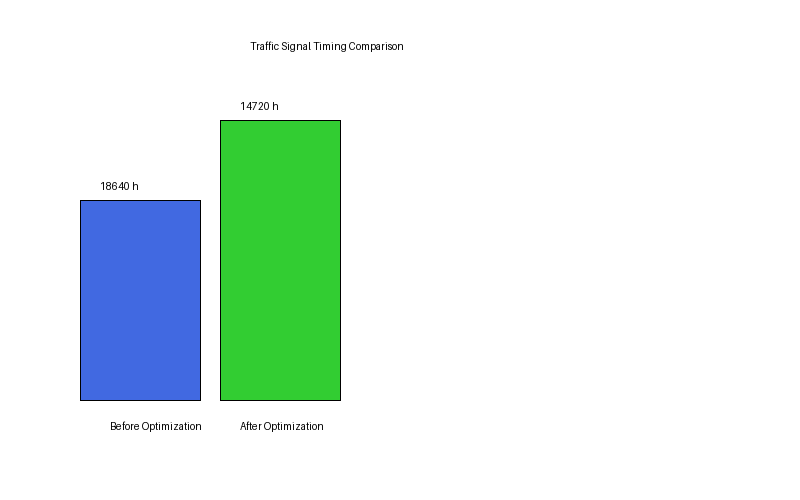
\includegraphics[width=0.85\textwidth]{figures/fig1.png}
  \caption{交叉口信号配时优化前后对比}
  \label{fig:1}
\end{figure}

\subsection{LSTM预测精度}

LSTM模型在测试集上的预测精度如表6所示。

\begin{table}[H]
  \centering
  \caption{表6: 预测步长}
  \label{tab:6}
  \begin{tabular}{cccc}
    \toprule
    预测步长 & RMSE(veh/5min) & MAE(veh/5min) & MAPE(\%) \\
    \midrule
    5 min & 12.3 & 9.1 & 6.8 \\
    10 min & 21.7 & 16.2 & 11.4 \\
    15 min & 34.5 & 26.8 & 18.3 \\
    \bottomrule
  \end{tabular}
\end{table}

5分钟预测精度达到93.2\%，能够满足实时交通管控的需求。预测结果拟合曲线如图2所示。

\begin{figure}[H]
  \centering
  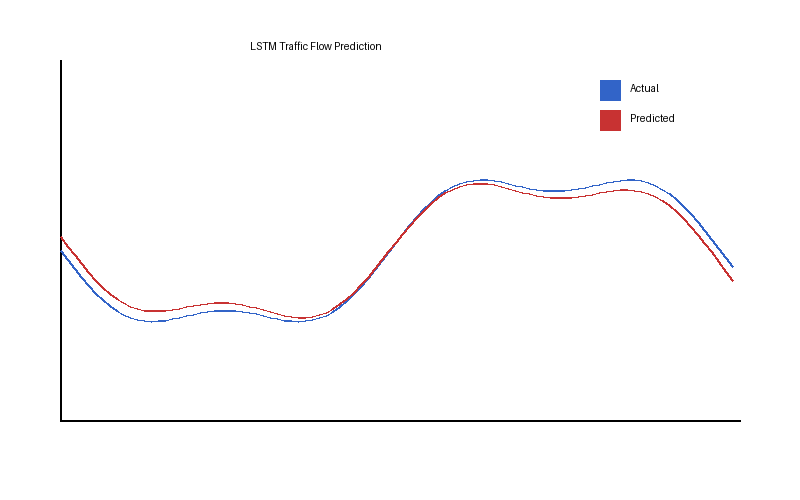
\includegraphics[width=0.85\textwidth]{figures/fig2.png}
  \caption{LSTM交通流预测拟合曲线}
  \label{fig:2}
\end{figure}

\section{模型评价与改进}

\subsection{模型优点}

（1）系统性：从微观到宏观构建了点—线—面—预测四层次一体化框架；

（2）可操作性：所有模型均有明确的求解算法，可直接应用于实际交通管控系统；

（3）可扩展性：各子模型相对独立，可根据实际需要灵活替换或升级；

（4）数据驱动：LSTM预测模型充分利用了交通大数据的特征，具有较强的自适应性。

\subsection{模型缺点}

（1）Greenshields线性模型假设速度-密度关系为线性，在实际中过于简化；

（2）遗传算法存在收敛速度慢、易陷入局部最优的问题；

（3）LSTM预测精度随预测步长增加而显著下降；

（4）未充分考虑非机动车与行人等混合交通流的影响。

\subsection{改进方向}

（1）采用Van Aerde、Newell等多参数速度-密度模型替代Greenshields模型；

（2）引入NSGA-II等多目标进化算法，同时优化延误、停车次数、油耗等指标；

（3）结合注意力机制与Transformer架构提升长时预测精度；

（4）考虑多模式交通（公交、地铁、共享单车）的协同优化。

\nocite{*}

\bibliography{ref}
